\begin{frame}[fragile]
  \frametitle{避不开的统计}
  \begin{block}{统计无处不在}
    在一个用事实说话的社会,我们接触到了越来越多的统计数据和资料:
    \begin{itemize}
      \item 耶鲁毕业生平均年收入25111美元 
      \item 普通美国人每天刷牙1.02次
      \item 钢铁公司职工平均周收入攀升了107\%
      \item 自从使用了多斯克牌牙膏,我们的蛀牙减少了23\%
      \item 低于智商平均数100的小孩智力有问题
      \item 一个四口之家的平均总收入为5004美元
      \item ……
    \end{itemize}
  \end{block}
  \pause
  \begin{block}{然而……}
    大量的统计数据、统计资料由于主、客观的原因被滥用,很难起到描述事实、传递信息的作用。相反,还往往对读者形成误导。
  \end{block}
\end{frame}

\begin{frame}
  \frametitle{说谎的统计数字}
  \begin{block}{质疑“平均工资”}
    \begin{itemize}
      \item 2004年,广州市职工平均工资为28237元。
      \item 市民普遍反映年工资收入基本达不到这个水平,有的甚至相距甚远。
    \end{itemize}
  \end{block}
  \pause
  \begin{block}{“谎言”的背后}
    \begin{itemize}
      \item 职工统计中有七类人员没有列入范围,而这部分人正属于收入较低的群体。
      \item 当数据的分布呈现正偏态时,均值往往偏离一般水平,并且高于一般水平。
    \end{itemize}
  \end{block}
\end{frame}

\begin{frame}[fragile]
  \frametitle{课程主旨}
  \begin{block}{统计 vs. 谎言 vs. 技能}
    \begin{itemize}
      \item 有3种谎言:谎言、糟糕透顶的谎言和统计资料。
      \item 使我们陷入麻烦的通常并非我们不知道的事情,而是那些我们知道得不确切的事情。
      \item 对于追求效率的公民而言,统计思维总有一天会和读写能力一样必要。
    \end{itemize}
  \end{block}
  \pause
  \vspace{-0.5em}
  \begin{block}{练就看穿统计资料的“火眼金睛”}
    对统计资料应该提出五个问题:
    \begin{enumerate}
      \item 谁说的
      \item 如何知道的
      \item 是否遗漏了什么
      \item 是否偷换了概念
      \item 资料是否有意义
    \end{enumerate}
  \end{block}
\end{frame}

\begin{frame}
  \frametitle{课程主旨}
  \begin{figure}
    \centering
    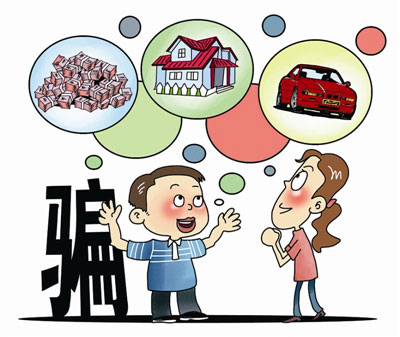
\includegraphics[width=0.4\textwidth]{c0.object.01.jpg}
    
\includegraphics[width=0.13\textwidth]{c0.object.03.jpg}
    
\includegraphics[width=0.35\textwidth]{c0.object.02.jpg}
  \end{figure}
  \begin{block}{对数据判断和接收的态度}
    如果一个人以种种肯定的立论开始,他必将终止于各种怀疑;但如果他愿意抱着怀疑的态度开始,那么他必将获得肯定的结论。
  \end{block}
\end{frame}

\begin{frame}
  \frametitle{参考教材}
  \begin{figure}
    \centering
    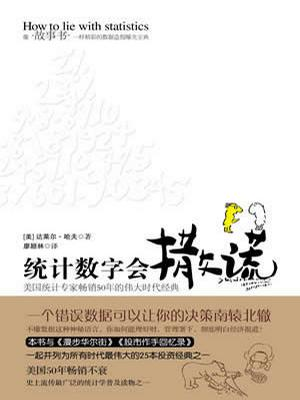
\includegraphics[width=2.8cm]{c0.book.01.jpg}\qquad
    
\includegraphics[width=2.8cm]{c0.book.02.jpg}\\
    
\includegraphics[width=2.6cm]{c0.book.03.jpg}\qquad
    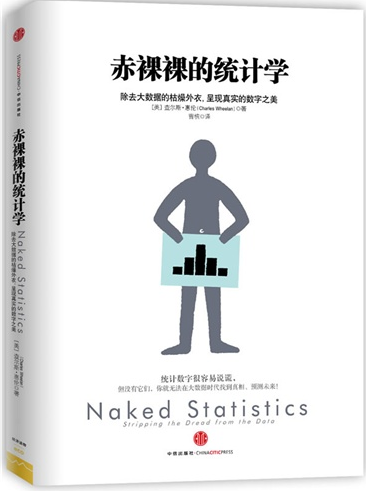
\includegraphics[width=3cm]{c0.book.04.png}
  \end{figure}
\end{frame}

\begin{frame}
  \frametitle{课外读物}
    \begin{block}{统计学与数据分析}
      \begin{multicols}{2}
      \begin{itemize}
         \item 《生活中的概率趣事》
         \item 《改变世界的134个概率统计故事》
         \item 《介绍丛书:统计学》
         \item 《漫画玩转统计学》
         \item 《漫画统计学》
         \item 《白话统计学》
         \item 《爱上统计学》
         \item 《从零开始读懂统计学》
         \item 《你一定爱读的极简统计学》
         \item 《深入浅出统计学》
         \item 《深入浅出数据分析》
        \end{itemize}
      \end{multicols}
    \end{block}
\end{frame}

\begin{frame}
  \frametitle{授课资料}
  \begin{figure}
    \centering
    
\includegraphics[width=0.55\textwidth]{qr.png}
  \end{figure}
  \begin{center}
    \href{https://github.com/Yixf-Education/course_Statistics_Story}{https://github.com/Yixf-Education/course\_Statistics\_Story}
  \end{center}
\end{frame}

\begin{frame}
  \frametitle{短片视频}
  \begin{figure}
    \centering
    
\includegraphics[width=0.55\textwidth]{c0.short.movie.png}
  \end{figure}
  \begin{center}
    \href{http://www.tudou.com/listplay/YUwEELLXLoI.html}{http://www.tudou.com/listplay/YUwEELLXLoI.html}
  \end{center}
\end{frame}

\begin{frame}
  \frametitle{课程安排}
  \begin{center}
  \alert{后9周(的前8周),每周二,晚上两节(18:00-20:00),西楼403}\\
  \vspace{0.2cm}
  \end{center}
  \begin{block}{授课内容}
    \begin{itemize}
      \item 抽样、均值、误差、趋势、图形、相关、技巧……
      \item 介绍基本的统计理念,(基本)不涉及统计术语/方法/公式
      \item 图说天下,谈天说地,评古论今
    \end{itemize}
  \end{block}
\end{frame}

\begin{frame}
  \frametitle{\alert{考核方式}}
  \begin{block}{考勤}
    \begin{itemize}
      \item 不点名,但随机提问
      \item 缺勤0次——优秀(及以下)
      \item 缺勤1次——良好(及以下)
      \item 缺勤2次——及格(及以下)
      \item 缺勤3次——不及格
    \end{itemize}
  \end{block}
  \pause
  \begin{block}{报告}
    \begin{itemize}
      \item 内容:自己关于某个(错误)统计数字/图形/资料/报道的看法
      \item 要求:电子版,~500字(一页纸),含信息来源、资料(的错误)分析等;抄袭——不及格
      \item 提交:yixfbio@gmail.com,课程名-学号-姓名-共享/保密.doc
      \item 示例:在Word里面撰写 $\rightarrow$ 重命名为“故事中的统计学-201600-张三-共享.doc” $\rightarrow$ 发送邮件 $\rightarrow$ 等待回复
    \end{itemize}
  \end{block}
\end{frame}

